\documentclass{ExcelAtFIT}
\usepackage[T1]{fontenc}
%\documentclass[czech]{ExcelAtFIT} % when writing in CZECH
%\documentclass[slovak]{ExcelAtFIT} % when writing in SLOVAK


%--------------------------------------------------------
%--------------------------------------------------------
%	REVIEW vs. FINAL VERSION
%--------------------------------------------------------

%   LEAVE this line commented out for the REVIEW VERSIONS
%   UNCOMMENT this line to get the FINAL VERSION
%\ExcelFinalCopy


%--------------------------------------------------------
%--------------------------------------------------------
%	PDF CUSTOMIZATION
%--------------------------------------------------------

\hypersetup{
	pdftitle={Paper Title},
	pdfauthor={Author},
	pdfkeywords={Keyword1, Keyword2, Keyword3}
}

%--------------------------------------------------------
%--------------------------------------------------------
%	ARTICLE INFORMATION
%--------------------------------------------------------

\ExcelYear{2018}

\PaperTitle{How to Write an Excellent Excel@FIT Paper}

\Authors{Adam Herout*}
\affiliation{*%
  \href{mailto:herout@fit.vutbr.cz}{herout@fit.vutbr.cz},
  \textit{Faculty of Information Technology, Brno University of Technology}}
%%%%--------------------------------------------------------
%%%% in case there are multiple authors, use the following fragment instead
%%%%--------------------------------------------------------
%\Authors{Jindřich Novák*, Janča Dvořáková**}
%\affiliation{*%
%  \href{mailto:xnovak00@stud.fit.vutbr.cz}{xnovak00@stud.fit.vutbr.cz},
%  \textit{Faculty of Information Technology, Brno University of Technology}}
%\affiliation{**%
%  \href{maildvora00@stud.fit.vutbr.cz}{xdvora00@stud.fit.vutbr.cz},
%  \textit{Faculty of Information Technology, Brno University of Technology}}

\Keywords{Evolutionary computation --- Neural Networks --- Linear Genetic Programming --- Robotics --- Robot evolution}

\Supplementary{\href{http://youtu.be/S3msCdn3fNM}{Demonstration Video} --- \href{http://excel.fit.vutbr.cz/}{Downloadable Code}}


%--------------------------------------------------------
%--------------------------------------------------------
%	ABSTRACT and TEASER
%--------------------------------------------------------

\Abstract{
Tato prace se zabyva navrhem a pouzitim frameworku vyuzivajici Evolucni Algoritmy, ktery bude pouzit pro hledani zpusobu rizeni pocitacoveho
modelu jednoducheho autonomniho robota. Tento model bude v pocitacove simulaci vykonavat netrivialni pohyb.
Pro řízení modelu robota jsou použity dva rozdílné přístupy.
První přístup je založen na instrukcích, odpovidajici Linearnimu Genetickemu Programovani.
Druhý přístup využívá feedforward neuronové sítě.
Oba pristupy jsou podrobeny nekolika experimentum, ktere overuji jejich vhodnost pro dany typ problemu.
Nasledne jsou pristupy vyhodnoceny a diskutovany vysledky s durazem na porovnani obou pristupu.
Vysledky prace potrvzuji, ze komplexnejsi chovani vyzaduje jistou miru samoadaptace(environment awarness) a ze je toto
mozne dosahnout obema zvolenymi pristupy.
}

\Teaser{
	\TeaserImage{placeholder.pdf}
	\TeaserImage{placeholder.pdf}
	\TeaserImage{placeholder.pdf}
}



%--------------------------------------------------------
%--------------------------------------------------------
%--------------------------------------------------------
%--------------------------------------------------------
\begin{document}

\startdocument


%--------------------------------------------------------
%--------------------------------------------------------
%	ARTICLE CONTENTS
%--------------------------------------------------------

%--------------------------------------------------------
%--------------------------------------------------------
%--------------------------------------------------------
%--------------------------------------------------------
\section{Introduction}

\textbf{[Motivation]} What is the raison d'\^{e}tre of your project? Why should anyone care? No general meaningless claims. Make bulletproof arguments for the importance of your work.

\todo{asi bych prevzal uvod do nejake robotiky}
V oblasti robotiky je velmi dulezita schopnost rychle a levne prototypovat mozna reseni.
K tomuto ucelu je velmi vhodne pouziti pocitacove modelovani a simulace.
V situaci, kdy mame navrzenou fyzickou stranku robota, nastava otazka, jak rychle prototypovat jeho rizeni.
Existuje mnoho moznosti realizace rizeni robota, lisici se v zavislosti na pozadavcich a povaze cinosti robota.
\todo{Citace, zdroje}
Rizeni robota muze byt zalozeno na instrukcich nejakeho imperativniho jazyka.
Mozne je take  pouziti neuronovych siti.
Dalsi z moznosti jsou ruzne planovaci algoritmy a systemy. \todo{citace, zdroje, terminologie}
Pro prototypovani je vyhodne mit nastroj, ktery je schopny hledat vyhodne zpusoby rizeni robota.
Evolutionary algorithms are good for this purpose, because they are applicable for a wide range of problems.~\cite{Eiben2015}

\textbf{[Problem definition]} What exactly are you solving? What is the core and what is a bonus? What parameters should a proper solution of the problem have? Define the problem precisely and state how its solution should be evaluated.

Hledame reseni pro problem, ktery je definovan takto.
Mame model jednoducheho robota, ktery je castecne inspirovany prirodou(mravenec). \todo{viz obr.}
Cilem prace je nalezt program(posloupnost instrukci) nebo konfiguraci neuronove site tak, aby model robota vykonaval dany netrivialni pohyb.
Hledame tedy jiste reseni.
Vybrane vzory pohybu jsou pohyb po primce a pohyb po spirale.
Hledani reseni probiha automatizovane s vyuzitim evolucnich algoritmu.
Algoritmy pomoci evoluce vyvijeji program, nebo neuronovou sit tak, aby se robot pohyboval po pozadovane trajektorii.
K vyhodnoceni uspesnosti reseni je pouzit fyzikalni simulator specializovany na simulaci robotu Mujoco[\todo{odkaz}].

\textbf{[Existing solutions]} Discuss existing solutions, be fair in identifying their strengths and weaknesses. Cite important works from the field of your topic. Try to define well what is the \textit{state of the art}. You can include a Section 2 titled ``Background'' or ``Previous Works'' and have the details there and make this paragraph short. Or, you can enlarge this paragraph to a whole page. In many scientific papers, \emph{this} is the most valuable part if it is written properly.
Soucasna reseni rizeni autonomnich robotu zahrnuji neuronove site\cite{Prabhu1996}, \cite{He2015}, fuzzy kontrolery\cite{Melendez2012}\cite{Saffiotti1997}


\textbf{[Our solution]} Make a quick outline of your approach -- pitch your solution.  The solution will be described in detail later, but give the reader a very quick overview now.
\phony{Lorem ipsum dolor sit amet, consectetur adipiscing elit. Morbi laoreet risus a egestas imperdiet. Ut egestas nibh non fermentum vestibulum. Nullam quis eleifend ex, sed maximus nisl. Mauris maximus non dolor id tristique. Nunc pulvinar congue gravida. Nullam lobortis viverra leo sed commodo. Nulla in elit congue, ullamcorper metus non, eleifend risus. Vivamus porttitor, ex nec porttitor pretium, libero turpis ultrices dui, eu efficitur ante ipsum vel justo. Vivamus nec nulla nisi. Aenean quis mauris vitae metus gravida congue.}

\textbf{[Contributions]} Sell your solution. Pinpoint your achievements. Be fair and objective.
\phony{Lorem ipsum dolor sit amet, consectetur adipiscing elit. Integer sit amet neque vel mi sodales interdum nec a mi. Aliquam eget turpis venenatis, tincidunt purus eget, euismod neque. Nulla et porta tortor, id lobortis turpis. Sed scelerisque sem eget ante interdum, vel volutpat arcu volutpat. Aliquam cursus, dolor a luctus. }


%--------------------------------------------------------
%--------------------------------------------------------
%--------------------------------------------------------
%--------------------------------------------------------
\section{Teoreticky uvod}
\label{sec:theory}
\todo{Zde bude kratky teoreticky uvod k EA a LGP}

%--------------------------------------------------------
%--------------------------------------------------------
%--------------------------------------------------------
%--------------------------------------------------------

\todo{zde se nekde musi vmestnat zakladni veci, tj. mame scenu, kde jsou referencni body}
\section{Framework architecture and implementation}
\label{sec:ArchitectureAndImplementation}
{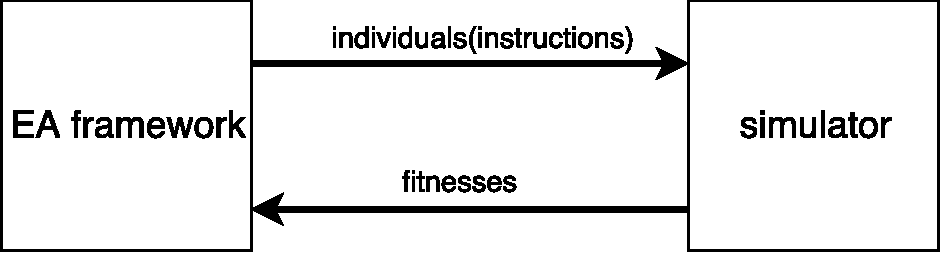
\includegraphics[height=5.8em]{top_level_architecture.pdf}
\todo{misto fitness psat o objective function?}
System je rozdelen na dve aplikace.
Hlavni aplikaci je EA framework, ktery zajistuje vsechnu praci s evoluci.
Druhou casti systemu je simulator Mujoco, ktery je doplnen vlastnim kodem, ktery zajistuje prevod instrukci na vstupy simulatoru a pocita fitness.
Propojeni techto dvou aplikaci je realizovano pres systemova volani pro spousteni procesu pres shell.
EA framework tedy pro kazdou generaci vytvori soubor, ktery obsahuje instrukce a spusti simulator.
Simulator nacte instrukce ze souboru, provede simulaci postupne pro vsechny sady instrukci a nasledne do jineho souboru ulozi hodnoty fitness.
EA framework pote tyto hodnoty fitness ze souboru precte a dale s nimi pracuje.

\subsection{dunno}
Rizeni robota je realizovano pomoci jednoduchych instrukci.
V simulatoru je zabudovat interpret, ktery je schopny tyto instrukce prevadet na signaly, ktere zpracovava simulator.
Tyto signaly rikaji, jaka sila se bude aplikovat v jednotlivych kloubech modelu robota.
Interpret pracuje pouze s celymi cisly, a to od -5 do 5 vcetne.

Interpret obsahuje predem dany pocet vnitrnich pametovych mist(vnitrni registry), ktere je mozne modifikovat za pouziti instrukci.
Interpret take obsahuje vystupni pametova mista(vystupni registry).
Kazdy vystupni registr je prirazen k jednomu kloubu robota.
Hodnoty v techto registrech jsou prevadeny na intenzitu sily, ktera bude v techto kloubech pusobit.

Program se sklada z instrukci, ktere meni stav vnitrnich registru a stav vnejsich registru.
Tyto instrukce jsou vypsany v (e.g. Table~\ref{tab:Instructions}) (e.g. Table~\ref{tab:ExampleTable})

Program je rozdelen do tri podprogramu - init, event a main.
Init program je proveden v nulovem case a to pouze po spusteni simulace.
Slouzi k nastaveni pocatecniho stavu vnitrnich registru. Jsou zde povoleny jen instrukce \todo{SRE?}

Dalsim podprogramem je event.
Ten je spousten pokazde, kdyz se model robota dostatecne priblizi k nekteremu z referencnich bodu(pro kazdy bod ale pouze jednou).
Vsechny instrukce jsou provedeny v nulovem case, stejne jako v init podprogramu.
Tento podprogram slouzi ke zmene vnitrich registru.
Jsou zde povoleny instrukce \todo{inc, dec?}

Hlavnim podprogramem je main.
Tento podprogram je provaden v nekonecne smycke.
Zde probiha kopirovani hodnot z vnitrnich registru do vystupnich registru.
Instrukce zde nejsou provadeny v nulovem case, ale casovy rozestup mezi nimi je 0.5 sekundy.
Jsou zde povoleny instrukce \todo{pro kopirovani z registru a naplneni registru konstantou}


\begin{table}[h]
	\caption{Instructions of the interpret}
\caption*{
%\vspace*{.8em}

Table of interpret instructions.
INC increments an internal register by a given constant.
DEC decrements an internal register by a given constant.
SOU copies an internal register value to a output register.
SOV copies a constant value to a output register.
SRE copies a constant to an internal register.
}
	\begin{tabular}{l|{c}|r}
		\textbf{Instruction}    & \textbf{Parameter 1} & \textbf{Parameter 2}    \\
		\hline
		INC                     & Internal register    & Constant        \\
		DEC                     & Internal register    & Constant        \\
		SOU                     & Internal register    & Output register \\
		SOV                     & Constant             & Output register \\
		SRE                     & Internal register    & Constant        \\
	\end{tabular}
	\label{tab:Instructions}
\end{table}


%--------------------------------------------------------
%--------------------------------------------------------
%--------------------------------------------------------
%--------------------------------------------------------
\section{Experiements}
\label{sec:Experiments}
\subsection{Experiment overview}
\todo{Zde bude popis experimentu - mravenec na primce? a na spirale}
\todo{Vsechny informace k experiemntu: tj. konfigurace GA, delka programu, rozdeleni na podprogramy(kolik kam), delka simulace}

\subsection{Results}
\todo{Zde budou prehledne vysledky experimentu - grafy, cisla, tabulky, obrazky, vsechno}
%--------------------------------------------------------
%--------------------------------------------------------
%--------------------------------------------------------
%--------------------------------------------------------

\section{Conclusions}
\label{sec:Conclusions}

\textbf{[Paper Summary]} What was the paper about, then? What the reader needs to remember about it?
Tato prace ukazala pouziti evolucnich algoritmu pro hledani programu pro rizeni robota. \todo{neco dalsiho}

\textbf{[Highlights of Results]} Exact numbers. Remind the reader that the paper matters.
\phony{Lorem ipsum dolor sit amet, consectetur adipiscing elit. Sed tempus fermentum ipsum at venenatis. Curabitur ultricies, mauris eu ullamcorper mattis, ligula purus dapibus mi, vel dapibus odio nulla et ex. Sed viverra cursus mattis. Suspendisse ornare semper condimentum. Interdum et malesuada fames ac ante ipsum.}

\textbf{[Paper Contributions]} What is the original contribution of this work? Two or three thoughts that one should definitely take home.
\phony{Lorem ipsum dolor sit amet, consectetur adipiscing elit. Praesent posuere mattis ante at imperdiet. Cras id tincidunt purus. Aliquam erat volutpat. Morbi non gravida nisi, non iaculis tortor. Quisque at fringilla neque.}

\textbf{[Future Work]} How can other researchers / developers make use of the results of this work?  Do you have further plans with this work? Or anybody else?
\phony{Lorem ipsum dolor sit amet, consectetur adipiscing elit. Suspendisse sollicitudin posuere massa, non convallis purus ultricies sit amet. Duis at nisl tincidunt, maximus risus a, aliquet massa. Vestibulum libero odio, condimentum ut ex non, eleifend.}

\section*{Acknowledgements}
I would like to thank my supervisor X. Y. for his help.

%--------------------------------------------------------
%--------------------------------------------------------
%--------------------------------------------------------
%	REFERENCE LIST
%--------------------------------------------------------
%--------------------------------------------------------
\phantomsection
\bibliographystyle{unsrt}
\bibliography{2018-ExcelFIT-ShortName-bib}

%--------------------------------------------------------
%--------------------------------------------------------
%--------------------------------------------------------
\end{document}
